% ------------------------------------------------------------------------
% Poster: Modelo de Poster para eventos de Lic. Inform.  
% 
% Template por Francisco Reinaldo 
%		(https://orcid.org/0000-0001-6161-6755)
%		(http://lattes.cnpq.br/7401534350061823)
% ------------------------------------------------------------------------
% Agradecimentos a Overleaf pela oportunidade 
% ------------------------------------------------------------------------

\def\footer#1{\def\insertfooter{#1}}
\documentclass[final]{beamer}

\usepackage[scale=1.150]{beamerposter}
\usetheme{MUWposter} 

%\logo{\pgfputat{\pgfxy(-13,108.5)}{\pgfbox[center,base]{\includegraphics[width=18cm]{logo_UTFPR.jpg}}}}  

\usepackage{multicol}
\usepackage{array}
%The following two are column definitions for the aknowledgements section
\newcolumntype{L}{>{\arraybackslash}m{22cm}}
\newcolumntype{S}{>{\arraybackslash}m{5cm}}
\usepackage{pgf}
%\usepackage{helvet}
\usepackage{mathtools}
\usepackage{amsmath, amsthm, amssymb, amsfonts}
\usepackage{exscale}
\usepackage{xcolor}
\usepackage{ushort}
\usepackage{setspace}
\usepackage{transparent}
\usepackage[square,numbers]{natbib}
\usepackage{url}
\usepackage{graphicx}
\bibliographystyle{abbrvnat}
\renewcommand{\vec}[1]{\ushort{#1}}
\renewcommand{\vec}[1]{\mathbf{#1}}
\definecolor{greenMUW}{RGB}{60,191,174}
\definecolor{blueMUW}{RGB}{17,29,79}
\definecolor{skinMUW}{RGB}{254,228,217}
\definecolor{hellblauMUW}{RGB}{95,180,229}
\usepackage{xcolor}
\usepackage{graphicx}
%-----------------------------------------------
%  START Set the colors
%  Uncomment to apply colors you want to use.
%-----------------------------------------------
\colorlet{themecolor}{greenMUW}
\usebackgroundtemplate{
\includegraphics[width=90cm,height=120cm]{MUW_green}}


%-----------------------------------------------
%  START Set the width of the columns
%-----------------------------------------------
\setlength{\paperwidth}{90cm} % A0 width: 46.8in
\setlength{\paperheight}{120cm} % A0 height: 33.1in
\newlength{\sepmargin}
\newlength{\sepwid}
\newlength{\onecolwid}
\newlength{\twocolwid}
\newlength{\threecolwid}
\usepackage{caption}
\captionsetup[figure]{labelformat=empty}%

% The following measures are used for 2 columns
\setlength{\sepmargin}{0.055\paperwidth} % Separation width (white space) between columns
\setlength{\sepwid}{0.03\paperwidth} % Separation width (white space) between columns
\setlength{\onecolwid}{0.425\paperwidth} % Width of one column
%\setlength{\twocolwid}{0.6\paperwidth} % Width of two columns

%-----------------------------------------------------------
% The following measures are used for 3 columns
%\setlength{\sepmargin}{0.06\paperwidth} % Separation width (white space) between columns
%\setlength{\sepwid}{0.02\paperwidth} % Separation width (white space) between columns
%\setlength{\onecolwid}{0.28\paperwidth} % Width of one column
%\setlength{\twocolwid}{0.58\paperwidth} % Width of two columns
%\setlength{\threecolwid}{0.88\paperwidth} % Width of three columns
%\setlength{\columnsep}{30pt}

%-----------------------------------------------
%  END Set the width of the columns
%-----------------------------------------------


%------------------------
\setbeamertemplate{title}[left]
\setbeamertemplate{frametitle}[default][left]
%\setmainfont{Georgia}

\title{Multi-Agent Reinforcement Learning Benchmark on Highway Environment for Autonomous Driving}
%small{Projeto  RED n.6, homologado, Edital 32/2014 PROGRAD - Produção de Recursos Educacionais Digitais]}\\}

\author{\textbf{Charbel ABI HANA}} % Author(s)

\institute{M1 International Track in Electrical Engineering - Université Paris-Saclay. Paris, France} % Institution(s)
%------------------------

\usepackage[absolute,overlay]{textpos}
  \setlength{\TPHorizModule}{1mm}
  \setlength{\TPVertModule}{1mm}

\begin{document}
%verificar width=10cm,height=10cm,keepaspectratio
\begin{textblock}{20}(580,30)

\includegraphics[scale=0.9]{images/evryyyy.png}
\end{textblock}

\begin{textblock}{20}(700,30)
\transparent{1}
\includegraphics[width=16cm]{images/logoParisSaclay.png}
\end{textblock}

%\begin{textblock}{20}(500,32.5)
%\includegraphics[width=10cm]{selos_ge2017.pdf}
%\end{textblock}

  \addtobeamertemplate{block end}{}{\vspace*{1ex}} % White space under blocks
  \addtobeamertemplate{block alerted end}{}{\vspace*{0ex}} % White space under highlighted (alert) blocks
  \setlength{\belowcaptionskip}{2ex} % White space under figures
  \setlength\belowdisplayshortskip{1ex} % White space under equations
  

\begin{frame}[t] 
\begin{columns}[t] 
\begin{column}{\sepmargin}\end{column}
\begin{column}{\onecolwid} % The first column
\vspace{1em}
  \begin{block}{Introduction}
\textbf{The domain of Reinforcement Learning has become a powerful learning framwork capable of learning
    complex policies in high dimensional environments. 
    Reinforcement learning models learn from an environment. The environment has a set of rules and is usually assumed to be deterministic. A reinforcement learning model interacts with the environment through an agent. The agent can perform actions that change its state in the environment.
\\}
\begin{figure}
    \vspace*{0.2cm}
    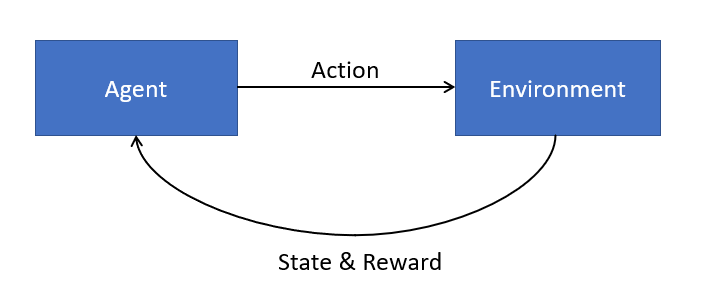
\includegraphics[width=0.6\linewidth]{images/rl_diag.png}
    \end{figure}

\textbf{Road tests for autonomous driving algorithms hasn't been widely applied due to safety reasons, therefore we use
    intricate simulators like OpenAI's Gym, PettingZoo, SUMO-RL and many others. In this project, we will benchmark known Reinforcement Learning
    models on a highway environment based on OpenAI Gym in which we simulate a multi-agent environment where multiple autonomously driven cars will navigate as fast as possible
    on a highway while avoiding collisions with human-driven cars.}

\end{block}
          
\begin{block}{The Environment}
\textbf{The environment is based on OpenAI's Gym library for simulation environments. It simulates autonmously-driven vehicles and human driven vehicles. We configure the environment to obtain 3 controlled vehicles
    and 10 human vehicles. 
}

\begin{figure}
\vspace*{0.2cm}
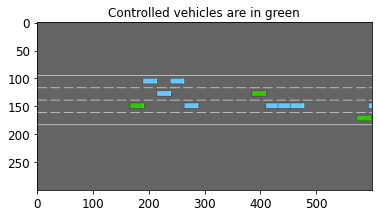
\includegraphics[width=0.6\linewidth]{images/highway-env.png}
\end{figure}

\end{block}    
          
\begin{block}{Action/Observation Space}
\textbf{The action space is configured to be discrete. The availability of the actions depends on the positioning of the agent
    in the environment. The actions that each RL agent in the envrionemnt can take are \textit{lane\_left},\textit{lane\_right},
    \textit{idle}, \textit{faster} and \textit{slower}.\\}
\textbf{We'll be using the \textit{KinematicObservation} which essentially is  $V*F$  array where $V$  
represents a list of nearby vehicles and $F$ represents the feature being the $x-y$  
positions and velocities. We can also add the vehicle's orientation. 
}

\begin{figure}[!tbp]
    \vspace*{0.2cm}
    \centering
    \begin{minipage}[b]{0.5\textwidth}
      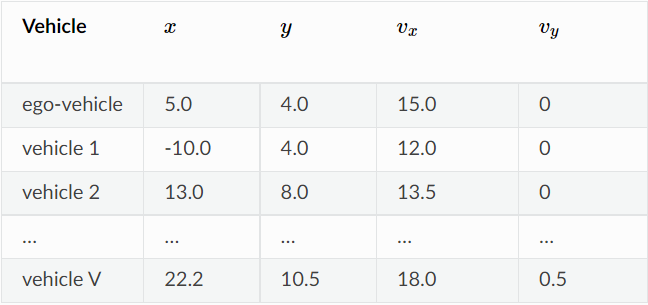
\includegraphics[width=\textwidth]{images/observation_space.png}
      \caption{Observation Space}
    \end{minipage}
    \hfill
    \begin{minipage}[b]{0.26\textwidth}
      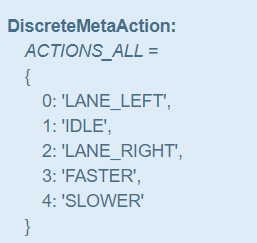
\includegraphics[width=\textwidth]{images/action_space.png}
      \caption{Action Space}
    \end{minipage}
  \end{figure}

\end{block}

\end{column}

\begin{column}{\sepwid}\end{column}
\begin{column}{\onecolwid} %The second column
\vspace{1em}

 \begin{block}{Reward}

\textbf{The general focus is on two features: a vehicle should progress quickly on the road and should avoid collisions. Thus, the reward function is often composed of a velocity term and a collision term:\\ 
\begin{equation}
    R(s,a) = a * \frac{v - {v}_{\min}}{{v}_{\max}-{v}_{\min}} - b * {collision}
\end{equation}
where  $v$, ${v}_{\min}$ and ${v}_{\max}$  are the current, minimum and maximum speed of the ego-vehicle respectively, and  $a$, $b$  are two configurable coefficients.}

 \end{block}
               
\begin{block}{Decentralized Algorithms}
    \begin{itemize}
        \item \textbf{IDQN - independent DQN agents, one per autonomously-driven car, each with convolution layers.}
        \begin{figure}[!ht]
            \vspace*{0.1cm}
            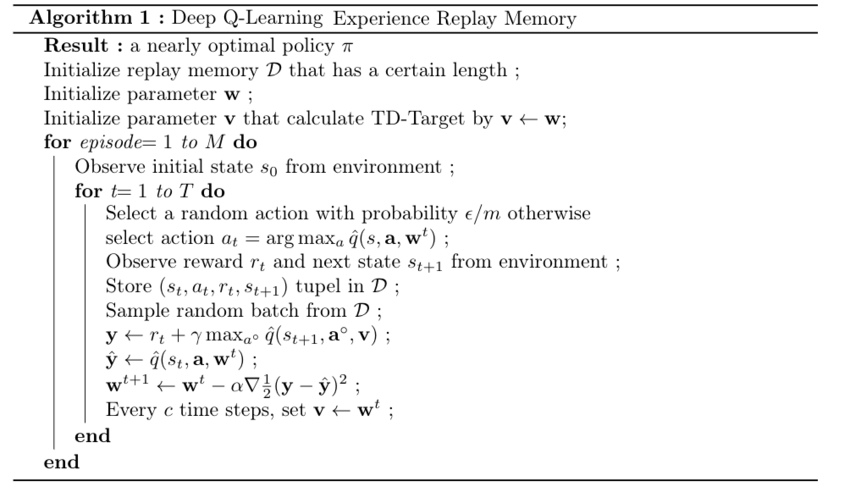
\includegraphics[width=0.7\linewidth, height=0.37\linewidth]{images/DQN-Algorithm.png}
        \end{figure}
        \item \textbf{IPPO - independent PPO agents with similar neural network as the DQN agents.}
        \begin{figure}[!ht]
            \vspace*{0.1cm}
            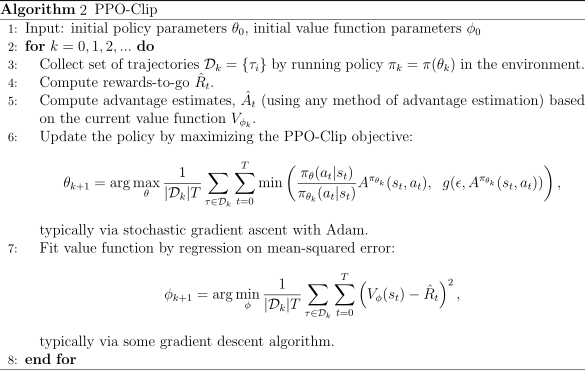
\includegraphics[width=0.7\linewidth, height=0.37\linewidth]{images/ppo_algorithm.png}
        \end{figure}
    \end{itemize}
 \end{block} 
 
\begin{block}{Results}
    \textbf{The metrics used to compare both algorithms was the score over an episode. The reward is noisy as it is highly dependant of model
    hyperparameters but an overall convergence can be seen.}

    \begin{figure}[!tbp]
        \vspace*{0.2cm}
        \centering
        \begin{minipage}[b]{0.4\textwidth}
          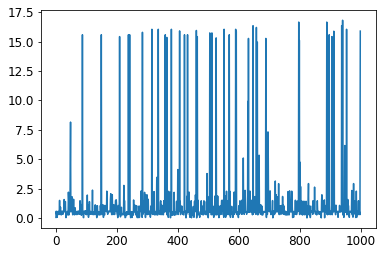
\includegraphics[width=\textwidth]{images/idqn-res.png}
          \caption{IDQN Model - Score vs Episodes}
        \end{minipage}
        \hfill
        \begin{minipage}[b]{0.4\textwidth}
          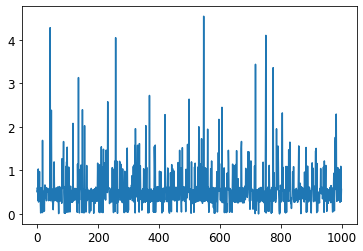
\includegraphics[width=\textwidth]{images/ppo_res.png}
          \caption{IPPO Model - Score vs Episodes}
        \end{minipage}
      \end{figure}
\end{block} 

\begin{block}{Future Improvements}
    \begin{itemize}
      \item \textbf{Add centralized algorithms where agents communicate with one centralized controller}
      \item \textbf{Extend environment to highway merging and intersection handling}
    \end{itemize}
\end{block} 

\end{column}
\begin{column}{\sepmargin} \end{column}
\end{columns} 
\end{frame} 
	
\end{document}


